%%% Local Variables:
%%% mode: latex
%%% TeX-master: t
%%% End:

\documentclass{article}

\usepackage{fullpage}
\usepackage[utf8]{inputenc}
\usepackage{listings}
\usepackage{caption}
\usepackage{subcaption}
\usepackage[svgnames]{xcolor}
\usepackage{amssymb}
\usepackage{amsmath}
\usepackage{fancyhdr}
\usepackage{lastpage}
\usepackage{parskip}
\usepackage{abstract}
\usepackage{gensymb}
\usepackage{url}
\usepackage{float}
\usepackage{enumitem}
\usepackage{amstext}
\usepackage{fancybox}
\usepackage{amsmath}
\usepackage{graphicx}
%\usepackage{subfigure}
\usepackage[bottom]{footmisc}
\usepackage{hyperref}
\usepackage{tikz}
\usepackage{makecell}
\usepackage{tabulary}
\usepackage{pdfpages}
\usepackage{verbatim}
\usepackage{tikz}
\usetikzlibrary{positioning}
\usetikzlibrary{arrows}
\pagenumbering{gobble}

\setcounter{secnumdepth}{3} % only chapter and sections will be numbered
\setcounter{tocdepth}{3}    % entries down to \subsubsections in the TOC

\definecolor{Brown}{cmyk}{0,0.81,1,0.60}
\definecolor{OliveGreen}{cmyk}{0.64,0,0.95,0.40}
\definecolor{CadetBlue}{cmyk}{0.62,0.57,0.23,0}
\definecolor{lightlightgray}{gray}{0.95}
\definecolor{lightgray}{gray}{0.85}
\definecolor{sh_comment}{rgb}{0.12, 0.38, 0.18}
\definecolor{sh_keyword}{rgb}{0.37, 0.38, 0.75}
\definecolor{sh_string}{rgb}{0.06, 0.10, 0.98}

\lstset{
basicstyle=\small\ttfamily,
stringstyle=\color{sh_string},
keywordstyle = \color{sh_keyword}\bfseries,
commentstyle=\color{sh_comment},
backgroundcolor=\color{lightlightgray},
frame=single,
rulecolor=\color{lightgray},
framesep=3pt,
numbersep=5pt,
xleftmargin=10pt,
xrightmargin=10pt,
showspaces=false,
showstringspaces=false,
tabsize=4,
aboveskip=5pt,
belowskip=5pt,
lineskip=2pt,
captionpos=b,
numbers=left,
numberstyle=\tiny,
stepnumber=1,
numbersep=100pt,
breaklines,
numbersep=5pt,
breakatwhitespace=false,
showspaces=false,
showtabs=false
}

\lstnewenvironment{cpp}[0]{
\lstset{language=C++,
}}
{}


\lstnewenvironment{assembly}[0]{
\lstset{language={[x86masm]Assembler},
}}
{}


\title{Operating System Notes}
\author{December 2014}
\date{}

\begin{document}

\maketitle
\tableofcontents
\pagebreak

\setcounter{page}{1}
\pagenumbering{arabic}

\section{Compiler optimization}
\emph{1. You can list and describe three source code transformations the compiler can perform to achieve higher performance.}

\begin{enumerate}
  \item \textbf{Loop optimization}: Move loop-invariant variables outside the loop.
  \item \textbf{Dead code elimination}
  \item \textbf{Common subexpression elimination}: $(x + y) / 3.0 - (x + y)\rightarrow temp = y+x;\;\; temp/3.0-temp$
  \item \textbf{Jump threading} when one jump directly to a second jump. If the second condition is a subset or inverse of the first, it can be eliminated, or threaded through the first jump.
  \begin{assembly}
10. a = SomeNumber();
20. IF a > 10 GOTO 50
...
50. IF a > 0 GOTO 100
...
  \end{assembly}
  Here the first jump can safely be modified to jump directly to line 100, as it the condition will always be true.
  \item \textbf{Instruction scheduling}: improve instruction-level parallelism. ``Simply'' put, avoid \emph{pipeline stalls} by rearranging the order of instructions. Pipeline stalls can be caused by structural hazards (processor resource limit), data hazards (output of one instruction needed by another instruction) and control hazards (branching).
  \item Replacing instructions with more efficient ones. For instance, x = x * 2 is likely faster performed by bitshifting
\end{enumerate}

Primarily optimizing either for (run) time or for space.


\section{Programming methodologies}
\emph{2. You can apply standard programming methodologies and tools such as test-driven development, build systems, debuggers.}

\begin{description}
\item[Test-driven development (TDD)] \ \\
Software development process. Cycle:
\begin{enumerate}
\item Write initially failing test defined desired functionality
\item Implement functionality, passing test
\end{enumerate}

\item[Build systems] \ \\
Automating common tasks as:
\begin{itemize}
\item Compiling computer source code into binary code
\item Packaging binary code
\item Running automated tests
\item Deploying to production systems
\item Creating documentation and/or release notes
\end{itemize}

\item[Debuggers] Process of finding and reducing number of bugs in program or part of hardware.
\end{description}


\section{Compilation toolchain}
\emph{3. You can explain the role of each component of a compilation toolchain used in system programming and how the components interact.}

\begin{enumerate}
	\item Source file(s) are handled by the preprocessor, which turn them into \textbf{translation units}:
	\begin{itemize}
		\item The preprocesser recursively includes files marked by \#include
		\item The preprocesser expands macros such as \#if, \#define, \#ifdef
	\end{itemize}
	Translation units consists of declarations and definitions.
	\item Each translation unit is then \emph{compiled} into object files
	\item Object files can then, together with (static) libraries, be linked into executables.
\end{enumerate}

\textbf{Remember} that there are both \emph{static} and \emph{dynamic} libraries. Static are linked into the executable, whereas dynamic can be changed (updated) with time (dynamic linked).

\textbf{Translation unit}
A translation unit consists of
\begin{itemize}
	\item Declarations
	\begin{itemize}
		\item Type
		\item Variable
		\item Function
	\end{itemize}

	\item Definition
	\begin{itemize}
		\item Variable
		\item Function
	\end{itemize}
\end{itemize}


\section{Memory leaks}
\emph{4. You can explain in your own words how memory leaks can occur in systems with dynamic memory management and give examples of two approaches to prevent them.}

\subsection{How they can occur}
\begin{itemize}
	\item In the C standard library, one can call \texttt{malloc()} to get a pointer to the memory of the requested size.
 If one deletes the pointers to the allocated data, without freeing the memory block before, this is a memory leak.

 	\item Memory fragmentation
\end{itemize}


\subsection{Strategies to prevent them}
\begin{itemize}$
	\item Garbage collection. Detect data objects that cannot be used by the program in the future, and free the resources occupied by these.
	\item Always add free after a malloc and then put code that uses the variable in between.
	\begin{cpp}
int *p = (int*) malloc ( sizeof(int) * n );
//Put code here..
free (p);
	\end{cpp}
	\item Never use allocated pointer for doing stuff. Instead use a copy and use that in code. Copy the pointer...
	\begin{cpp}
int *p_allocated = (int*) malloc ( sizeof(int) * n );
int *p_copy = p_allocated;
// do your stuff with p_copy, not with p_allocated!
// e.g.:
while (n--) { *p_copy++ = n; }
...
free (p_allocated);
	\end{cpp}
\end{itemize}


\section{Memory mapped I/O vs. I/O-instructions}
\emph{5. You can explain the difference between communicating with an I/O device using memory mapped I/O or I/O instructions.}
%%% Local Variables:
%%% mode: latex
%%% TeX-master: "../cheat-sheet"
%%% End:

% \emph{5. You can explain the difference between communicating with an I/O device using memory mapped I/O or I/O instructions.}

\textbf{Memory mapped I/O}: A device's memory is mapped to the CPU's memory address space, ie. the device's memory is manipulated in exactly the same way as regular memory.

\textbf{I/O instructions}: Processes can use I/O instructions, such as the \texttt{IN} and \texttt{OUT} instructions in the \texttt{x86} instruction set. Those two transfer data between I/O devices and registers/memory through the I/O ports of the CPU.



\section{CPU Terminology}
\label{cpu-term}
\emph{6. You can explain in your own words the following terms: processor, register, program counter, cache, I/O device, instruction set architecture.}
%%% Local Variables:
%%% mode: latex
%%% TeX-master: "cheat-sheet"
%%% End:

\begin{figure}[H]
  \centering
  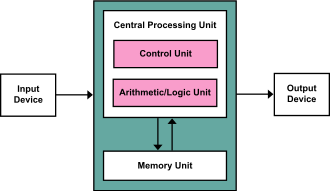
\includegraphics[width=8.0cm]{images/330px-Von_Neumann_Architecture.png}
  \caption{Von Neumann Architecture}
\end{figure}

\subsection{Processor}
There are different kinds of processors, the most widely used are
\begin{itemize}
	\item General purpose central processing units (CPUs, used in PCs)
	\item ASIC (application-specific integrated circuit)
	\item GPU (graphics processing units)
\end{itemize}

Operates in \textbf{cycles} (see~\nameref{sec:cpu-func} for details):
\begin{itemize}
	\item Fetch instruction (using the PC/IP)
	\item Decode instruction (there are different \emph{addressing modes})
	\item Execute - Control Unit and ALU (Arithmetic/Logic Unit)
\end{itemize}
(This is the so-called three-stage pipeline. There is also the modern superscalar CPU (see page 21 in DJ Tanenbaum's book))

\textbf{Word size} - Modern PCs use a word-size of 64 bits. Embedded systems using microcontrollers often have a smaller word size (modern ones have down to 8 bit)

\subsection{Register}
A processor register is a small amount of storage available as part of a digital processor, such as a CPU. Such registers are (typically) addressed by mechanisms other than main memory and can be accessed faster.


\begin{figure}[H]
  \centering
  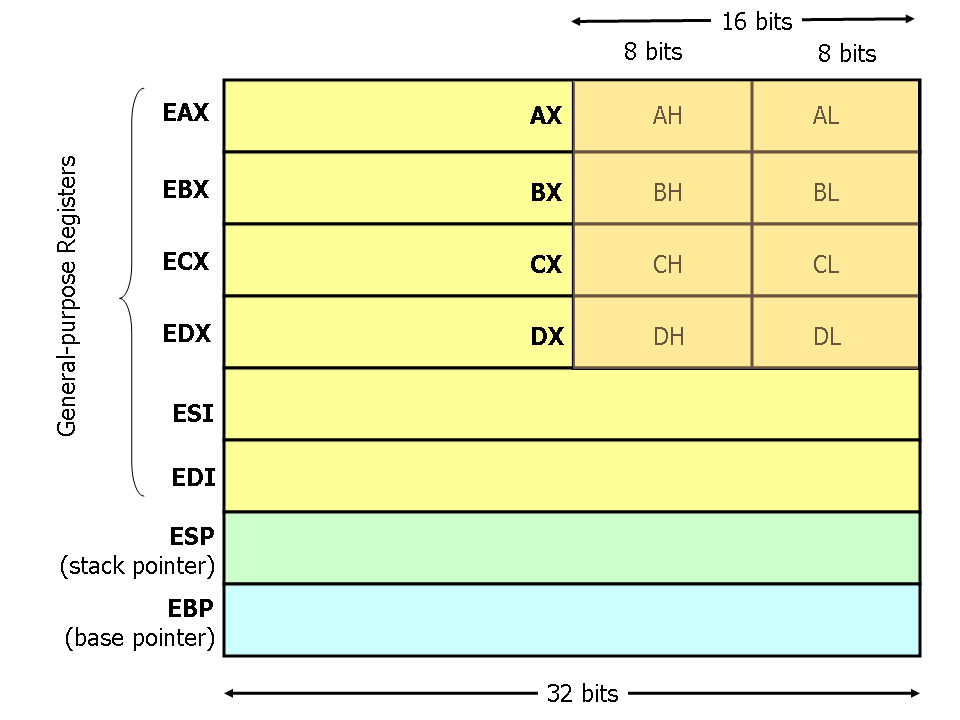
\includegraphics[width=8.0cm]{images/x86-registers}
  \caption{An overview of the registers (x86): }
\end{figure}

\subsection{Program counter / instruction pointer (PC/IP)}
A processor register that indicates where a computer is in its program sequence.

\subsection{Cache}
A CPU cache is used to reduce the average time to access data from the main memory. The cache is a smaller, faster memory which stores copies of the data from frequently used main memory locations.

In modern CPU's there are typically two \emph{layers of caches}, \textbf{L1} and \textbf{L2}. L1 cache is inside the CPU and feeds decoded instructions into the CPU's execution process. L2 cache holds several megabytes of recently used memory words. It is slower than L1, due to its size. Accessing L1 takes 1 cycle and acessing L2 takes 1 or 2 cycles.

On multicore chips, the placement of the L2 cache can vary. A single L2 cache can be shared by all the cores (intel).  This requires a more complicated cache controller. Another design is to give every core its own L2 cache (AMD). This is difficult to keep consistent.

\subsubsection{Cache cohorence}
A protocol for managing the caches of a multiprocessor system so that no data is lost or overwritten before the data is transferred from a cache to the target memory.

When multiple processors with separate caches share a common memory, it is necessary to keep the caches in a state of coherence by ensuring that any shared operand that is changed in any cache is changed throughout the entire system. This is done in either of two ways~\footnote{\url{http://www.webopedia.com/TERM/C/cache_coherence.html}}; through a directory-based or a snooping system:
\begin{enumerate}
\item In a directory-based system, the data being shared is placed in a common directory that maintains the coherence between caches. The directory acts as a filter through which the processor must ask permission to load an entry from the primary memory to its cache. When an entry is changed the directory either updates or invalidates the other caches with that entry.
\item In a snooping system, all caches on the bus monitor (or snoop) the bus to determine if they have a copy of the block of data that is requested on the bus. Every cache has a copy of the sharing status of every block of physical memory it has.
\end{enumerate}
Cache misses and memory traffic due to shared data blocks limit the performance of parallel computing in multiprocessor computers or systems. Cache coherence aims to solve the problems associated with sharing data.

\subsection{I/O device}
TODO

\subsection{Instruction set architecture (ISA)}
Well-defined software/hardware interface.

\begin{itemize}
	\item Functional definition - Operations and storage locations supported by hardware. With Intel's Ivy Bridge chip-architecture came the operation RdRand for instance, which is an operation that returns a hardware-generated random number.
	\item Documentation of how to use the instructions (see ABI below?).
\end{itemize}

(TODO: application binary interface (ABI). I believe this is contained within ISA. This defines the calling conventions for the architecture - for instance how system calls are carried out)


\begin{figure}[H]
  \centering
  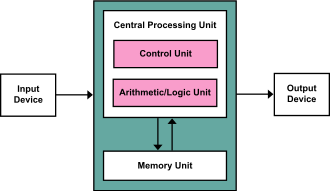
\includegraphics[width=8.0cm]{images/330px-Von_Neumann_Architecture.png}
  \caption{Von Neumann Architecture}
\end{figure}


\subsection{Processor}
There are different kinds of processors, the most widely used are
\begin{itemize}
	\item General purpose central processing units (CPUs, used in PCs)
	\item ASIC (application-specific integrated circuit)
	\item GPU (graphics processing units)
\end{itemize}

Operates in \textbf{cycles}:
\begin{itemize}
	\item Fetch instruction (using the PC/IP)
	\item Decode instruction (there are different \emph{addressing modes})
	\item Execute - Control Unit and ALU (Arithmetic/Logic Unit)
\end{itemize}
(This is the so-called three-stage pipeline. There is also the modern superscalar CPU (see page 21 in DJ Tanenbaum's book))

\textbf{Word size} - Modern PCs use a word-size of 64 bits. Embedded systems using microcontrollers often have a smaller word size (modern ones have down to 8 bit)

\subsection{Register}
A processor register is a small amount of storage available as part of a digital processor, such as a CPU. Such registers are (typically) addressed by mechanisms other than main memory and can be accessed faster. 


\begin{figure}[H]
  \centering
  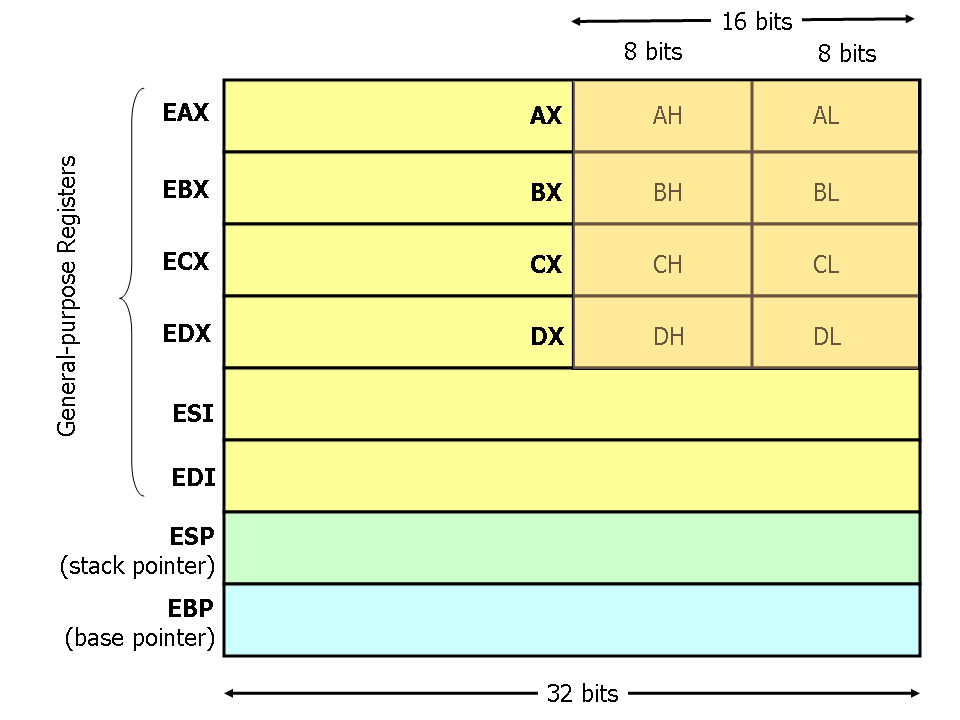
\includegraphics[width=8.0cm]{images/x86-registers}
  \caption{An overview of the registers (x86): }
\end{figure}

\textbf{General purpose registers} (GPRs) can be accessed by the programmer, usually there are 8, and in modern X86-64 processors there are 16 GPRs \footnote{\url{http://en.wikipedia.org/wiki/X86-64}}. In some RISC-processors \footnote{Reduced instruction set computing} there are 32 GPRs and in IA-64 (Intel Itanium architecture) there are 128 GPRs.


\subsection{Program counter / instruction pointer (PC/IP)}
A processor register that indicates where a computer is in its program sequence.

\subsection{Cache}
{\bf General:} A CPU cache is a cache used by the central processing unit (CPU) of a computer to reduce the average time to access data from the main memory. The cache is a smaller, faster memory which stores copies of the data from frequently used main memory locations.

In modern CPU'S there are typically two layers of caches, L1 and L2. L1 cache is inside the CPU and feeds decoded instructions into the CPUs execution process. L2 cache holds several megabytes of recently used memory words. It is slower than L1, due to its size. Accessing L1 takes 1 cycle and acessing L2 takes 1 or 2 cycles.

On multicore chips, the placement of the L2 cache can vary. A single L2 cache can be shared by all the cores (intel).  This requires a more complicated cache controller. Another design is to gice every core  its own L2 cache (AMD). This is difficult to keep consistent.

\subsubsection{Cache cohorence}
A protocol for managing the caches of a multiprocessor system so that no data is lost or overwritten before the data is transferred from a cache to the target memory. 


When multiple processors with separate caches share a common memory, it is necessary to keep the caches in a state of coherence by ensuring that any shared operand that is changed in any cache is changed throughout the entire system. This is done in either of two ways: 

through a directory-based or a snooping system. In a directory-based system, the data being shared is placed in a common directory that maintains the coherence between caches. The directory acts as a filter through which the processor must ask permission to load an entry from the primary memory to its cache. When an entry is changed the directory either updates or invalidates the other caches with that entry. In a snooping system, all caches on the bus monitor (or snoop) the bus to determine if they have a copy of the block of data that is requested on the bus. Every cache has a copy of the sharing status of every block of physical memory it has.
Cache misses and memory traffic due to shared data blocks limit the performance of parallel computing in multiprocessor computers or systems. Cache coherence aims to solve the problems associated with sharing data.






\subsection{I/O device}

\subsection{Instruction set architecture (ISA)}
Well-defined software/hardware interface.

\begin{itemize}
	\item Functional definition - Operations and storage locations supported by hardware. With Intel's Ivy Bridge chip-architecture came the operation RdRand for instance, which is an operation that returns a hardware-generated random number.
	\item Documentation of how to use the instructions (see ABI below?).
\end{itemize}

(TODO: application binary interface (ABI). I believe this is contained within ISA. This defines the calling conventions for the architecture - for instance how system calls are carried out)


\section{CPU Functionality}
\label{sec:cpu-func}
\emph{7. You can explain the basic workings of a processor and outline the steps involved in executing an instruction.}
%%% Local Variables:
%%% mode: latex
%%% TeX-master: "../cheat-sheet"
%%% End:

The processors execution of an instruction can be broken down into the following steps~\footnote{\url{http://www.howthecomputerworks.com/cpu/instruction-cycle/}}:
\begin{enumerate}
\item \textbf{Fetch} the instruction From RAM
\item \textbf{Decode} the instruction.
\item \textbf{Execute} the instruction.
\item \textbf{Fetch} any other memory needed to finish the executing the instruction.
\item \textbf{Retire}. Finish and write any memory that needs to be written.
\end{enumerate}

Also simply called the \emph{three-stage pipeline}, if one merges the last three steps. This is also the modern superscalar CPU (see p. 21 in Tanenbaum).

\begin{figure}[H]
  \centering
  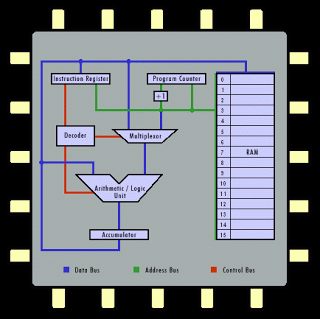
\includegraphics[scale=0.5]{images/cpu}
  \caption{Components of a simple CPU}
\end{figure}

\subsection{Fetch}
The CPU has a spacial register, the \textbf{program counter}, which contains the address of the next instruction to be executed.

After the CPU finishes executing the instruction, the register is updated to point to the next instruction. There is an exception when the CPU executes a branch instruction it will change the instruction pointer register to reflect the new address its supposed to jump to.

\subsection{Decode}
The \emph{decoder} component is responsible for figuring out what the instruction is supposed to do.

\subsection{Execute}
After the decoder sent the instruction to the proper unit, it is now the job of that unit to execute the instruction whatever that instruction maybe. E.g. an \texttt{add} instruction will be sent to the ALU.

\subsection{Fetch some more}
The execution unit may not always have all the necessary data to execute it sometime must fetch other data. This step is not always necessary.

\subsection{Retire}
Store what ever result and update the instruction pointer.



\section{Interrupts}
\emph{8. You can explain in your own words how interrupts are handled in the processor.}

When the processor gets interrupted, it
\begin{enumerate}
	\item Halts execution of the current thread
	\item Stores the current state (TODO: the book says that this ranges from storing only the IP-register, to storing \emph{all} registers of the thread).
	\item Executes interrupt handler
	\item Resumes thread execution
\end{enumerate}

Two types of interrupts:
\begin{itemize}
	\item \textbf{Hardware} - when a disk-read, keyboard input, clock (timing), scanned document is ready. Sent via the Bus.
	An Interrupt Controller handles this and issues interrupt for CPU.
	(if there are several HW-interrupts sent simultaneously, the ones with lower priorities keep sending the signal)

	\item \textbf{Software} - Either when an `interrupt instruction' is executed, or when an exception is thrown. (exceptions can be from other processors as well!)

\end{itemize}

The halting of execution and storing of state is much more complex on modern, superscalar CPUs (see page 21 in DJ Tanenbaum's)


\section{Indirect addressing (assembly)}
\emph{9. You can show with assembly code how the stack pointer, or a general purpose register, can be used to perform indirect addressing of data structures.}
%%% Local Variables:
%%% mode: latex
%%% TeX-master: "../cheat-sheet"
%%% End:

% 9. You can show with assembly code how the stack pointer, or a general purpose register, can be used to perform indirect addressing of data structures.

Consider
\begin{lstlisting}[language=C]
struct person {
  double height;
  int    age;
}

struct person turing = (struct person*)malloc(sizeof(struct person));
turing->age = 40;
turing->name = "Alan Turing";
\end{lstlisting}

We can now use indirect addressing to access the fields of the struct:

\begin{lstlisting}[language={[x86masm]Assembler}]
; eax now holds the address of `turing'
mov turing, %eax

; mov 1.0 to the first field of the struct (the double literal is not valid assembly)
mov $1.0, (%eax)

; mov 2 to the second field which is offset by 8 bytes (size of the double)
mov $2, 8(%eax)
\end{lstlisting}


Generally:
\begin{description}
\item[Indirect addressing:] \texttt{(\%eax)}
\item[Base pointer addressing:] \texttt{4(\%eax)}
\end{description}

The general form of memory address references is this:

\texttt{ADDRESS\_OR\_OFFSET(\%BASE\_OR\_OFFSET,\%INDEX,MULTIPLIER)}

\texttt{FINAL ADDRESS = ADDRESS\_OR\_OFFSET + \%BASE\_OR\_OFFSET + MULTIPLIER * \%INDEX}

See Bartlett chapter 3



\section{Memory hierarchy}
\emph{10. You can draw a figure showing how the memory hierarchy of a modern computer with the processor(s), cache levels, memory and storage}

\begin{center}
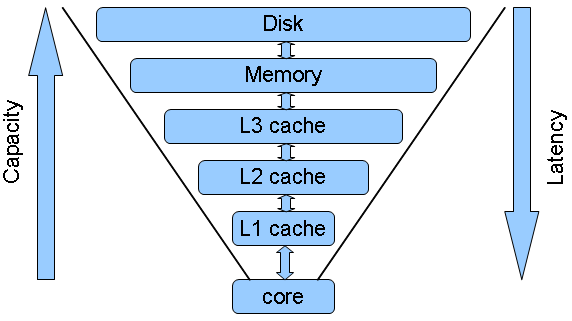
\includegraphics[width=5.0cm]{images/cpu_cache_structure.png}
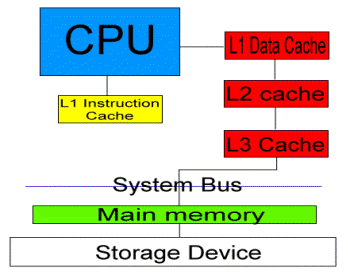
\includegraphics[width=5.0cm]{images/CPU-Cache-System.png}

Simplified overviews of CPU, registers, caches and memory
\end{center}

\emph{L1} is often local for each CPU, whereas \emph{L2} and/or \emph{L3} are/is often shared between multiple CPUs.

\emph{Extremely} important: When you draw the storage, remember to draw it as a cylinder\footnote{due to historical reasons}!


\section{Interrupt handler}
\emph{11. You can write pseudocode showing how to implement an interrupt handler.}
TODO


\section{Cache performance}
\emph{12. You can demonstrate with pseudo code how the memory access pattern of a program can greatly influence cache performance.}
%%% Local Variables:
%%% mode: latex
%%% TeX-master: "../cheat-sheet"
%%% End:

By avoiding cache misses (thus increasing cache hits) we can speed up memory lookups. When the CPU fetches memory it will fetch nearby elements into the cache as well because they are typically used together. If we fetch memory from scattered places its unfriendly for the cache.

For instance, iterating a two-dimensional array:

\begin{lstlisting}
nums = [[1, 2],
        [3, 4]]
// consider that `nums' this stored in memory as [1, 2, 3, 4]
\end{lstlisting}

If we iterate column-wise, and the cache fetches a single element ahead we get something like

\begin{lstlisting}
for col = 0 to 1:
    for row = 0 to 1:
        print nums[row][col]
\end{lstlisting}

This will result in accesses in this order: \texttt{nums[0][0] (1), nums[1][0] (3), nums[0][1] (2), nums[1][1] (4)}. If the CPU fetches and caches one address ahead then the first memory access fetches \texttt{nums[0][0] (1)} and caches \texttt{nums[0][1] (2)} but the next fetch is actually \texttt{nums[0][0] (3)} which results in a cache miss.

We can get two cache hits and two memory lookups instead of four memory lookups if we iterate row-wise instead!



\section{Privilege levels}
\emph{13. You can explain the concept of privilege levels and show three examples of operations which should be permitted only at the most privileged level.}
% 13. You can explain the concept of privilege levels and show three examples of operations which should be permitted only at the most privileged level.
Processes run under privilege level from 0 (most privileged) through 3 (least privileged). The assigned level controls what resources the process has access to, such as memory, IO, special instructions. Kernel code runs in ring 0 and general user programs run in level 3, all levels are not always used (for instance 1 and 2 are unused in Linux). Level 0 is essentially kernel mode. Current privilege level is stored in the \texttt{CPL} register.

Operations only permitted in level 0 (many of these are just system calls)
\begin{itemize}
\item Process creation
\item Process termination
\item Disable interrupts
\item Modify memory map (virtual memory)
\item File writing
\item File reading
\end{itemize}

%%% Local Variables:
%%% mode: latex
%%% TeX-master: "cheat-sheet"
%%% End:



\section{Message passing}
\emph{14. You can explain in your own words and in text and with your own commented examples, how message passing can be used to coordinate processes.}
% 14. You can explain in your own words and in text and with your own commented examples, how message passing can be used to coordinate processes.

Message passing in its simplest form is given by the two constructs \texttt{send} and \texttt{receive}, which could have signatures similar to

\begin{lstlisting}
void send(int process_id, string msg)
string receive(int process_id)
\end{lstlisting}

The semantics of the operations differ, for instance calling \texttt{receive} before \texttt{send} could either block until a message is available or return an error. If \texttt{recieve} waits for a call to \texttt{send} and vice versa it is called a \textbf{rendezvous} implementation.

An \textbf{important} issue to consider is how to establish connection between sender and receiver. It could be via a lookup by process name, hardcoded, manually set by user, via network names, stdin/stdout etc.

See figure~\ref{fig:msg-passing}: Code example from Tanenbaum p. 143
\begin{figure}[h]
  \centering
  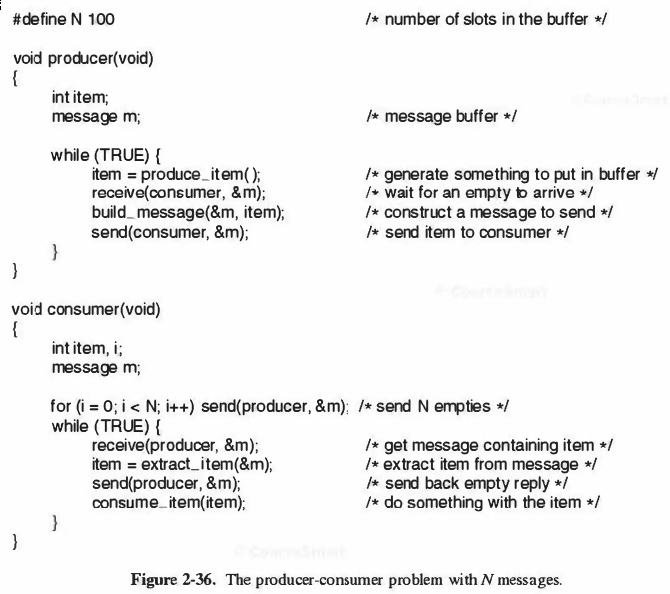
\includegraphics[width=0.8\textwidth]{images/message_passing}
  \caption{Producer/consumer via message example. From Tanenbaum.}
  \label{fig:msg-passing}
\end{figure}

%%% Local Variables:
%%% mode: latex
%%% TeX-master: "cheat-sheet"
%%% End:



\section{Kernel types}
\emph{15. You can explain in your own words the differences between a monolithic operat-
ing system, a micro-kernel operating system, and an exo-kernel based operating
system.}
%%% Local Variables:
%%% mode: latex
%%% TeX-master: "cheat-sheet"
%%% End:

\subsection{Monolithic}
\begin{itemize}
\item Entire operating system is working in kernel mode.
\item Defines a high-level virtual interface over computer hardware.
\item A set of primitives or system calls implement all operating system services such as process management, concurrency, and memory management.
\item Device drivers can be added to the kernel as modules.
\end{itemize}

\subsection{Microkernel}
\begin{itemize}
\item Near-minimum amount of software that can provide the mechanisms needed to implement an OS.
\item Mechanisms include low-level address space management, thread management, and inter-process communication (IPC).
\item Microkernel is the only software executing in kernel mode.
\item Other functions, such as device drivers, protocol stacks and file systems, are removed from the microkernel to run in user mode.
\item Focus on stability and security.
\item ``Program becomes the OS''
\end{itemize}

\begin{figure}[H]
  \centering
  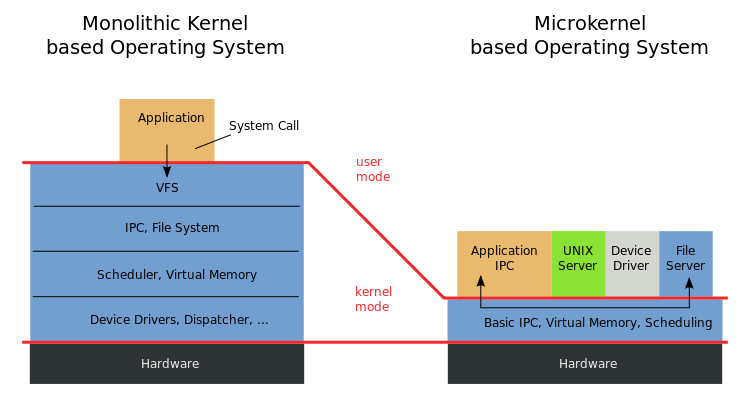
\includegraphics[scale=0.5]{images/mono-microkernel.png}
  \caption[Caption for LOF]{Overview of exo-kernel\footnotemark}
\end{figure}
\footnotetext{\url{https://en.wikipedia.org/wiki/Microkernel\#mediaviewer/File:OS-structure.svg}}

\subsection{Exokernel}
\begin{itemize}
\item Force as few abstractions as possible on developers, enabling them to make as many decisions as possible about hardware abstractions.

\item Tiny, since functionality is limited to ensuring protection and multiplexing of resources.

\item The kernel only ensures that the requested resource is free, and the application is allowed to access it.

\item Allows direct access to hardware from user space programs
\end{itemize}

\begin{figure}[H]
  \centering
  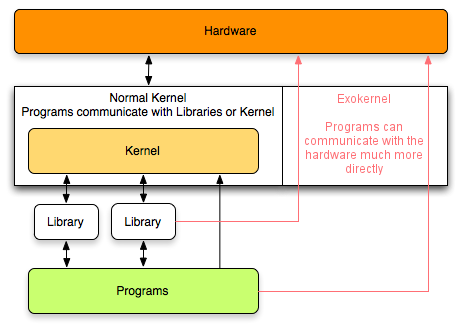
\includegraphics[scale=0.5]{images/exokernel.png}
  \caption[Caption for LOF]{Overview of exo-kernel\footnotemark}
\end{figure}
\footnotetext{\url{https://en.wikipedia.org/wiki/Exokernel\#mediaviewer/File:Exokernel\_revised(english).png}}



\section{Uni-processor system}
\emph{16. You can explain in your own words how multiple processes can share the same CPU.}
This is possible by context switching between the execution of the processes or threads (this is called \textbf{multitasking}). The context switch stores the current state of the process, so that the execution of it can be resumed at a later point in time.

This is most likely implemented with a preemptive scheduler on PCs, as programs would otherwise be able to hold on to the CPU. So the scheduler decides when to switch between processes.

\begin{center}
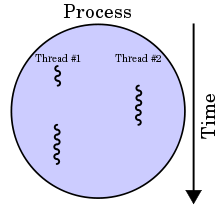
\includegraphics[width=5.0cm]{images/220px-Multithreaded_process.png}

A process with two threads - run on a single CPU
\end{center}

The above can also be performed between several processes, and thus a single CPU can execute several processes ``at the same time'' (at least it might appear so to the user).


\section{Multi-processor system}
\emph{17. You can explain in your own words how multiple processes can share a set of CPUs.}
With multiple CPUs one can, instead of switching out a running process to let another run, simply run the other process on another CPU.

Given the individual process address space and individual call stack for each thread, multiple processes are able to run in parallel on several CPUs without affecting the states of one another.


\section{Thread states}
\emph{18. Assume a thread can be in three different states: running, blocked, ready. You can draw a diagram of your own showing the transitions between states and explain in text and in your own words what each transition means.}
%%% Local Variables:
%%% mode: latex
%%% TeX-master: "cheat-sheet"
%%% End:

When a process blocks, it does so because logically it cannot continue, typically because it is waiting for input that is not yet available.

It is also possible for a process that is conceptually ready and able to run to be stopped because the operating system has decided to allocate the CPU to another process for a while.

These two conditions are \emph{completely different}. In the first case, the suspension is inherent in the problem (you cannot process the user' s command line until it has been typed). In the second case, it is a technicality of the system (not enough CPUs to give each process its own private processor).

The three possible states:
\begin{description}
\item[Running] Actually using the CPU at that instant
\item[Ready] Runnable; temporarily stopped to let another process run
\item[Blocked] Unable to run until some external event happens
\end{description}

\begin{figure}[H]
  \centering
  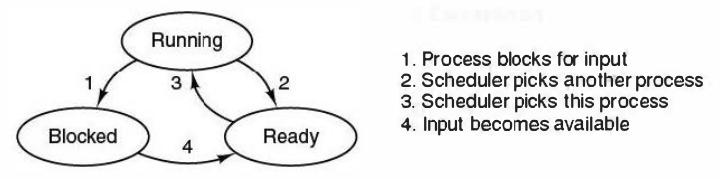
\includegraphics[scale=0.5]{images/thread_life}
  \caption{Transition diagram of thread states}
\end{figure}



\section{Operating system stack}
\emph{19. Given a schematic overview of the software stack of an operating system, you can label, in the diagram, key system parts. You can also explain in your own words and in text the purpose of those parts.}


\begin{figure}[H]
  \centering
  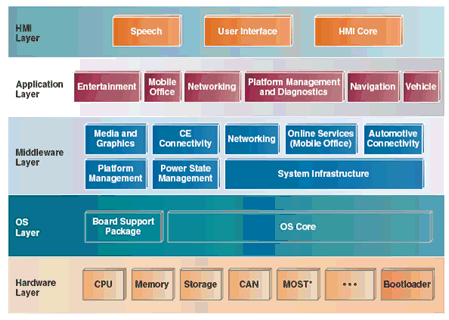
\includegraphics[width=8.0cm]{images/os-stack.png}
  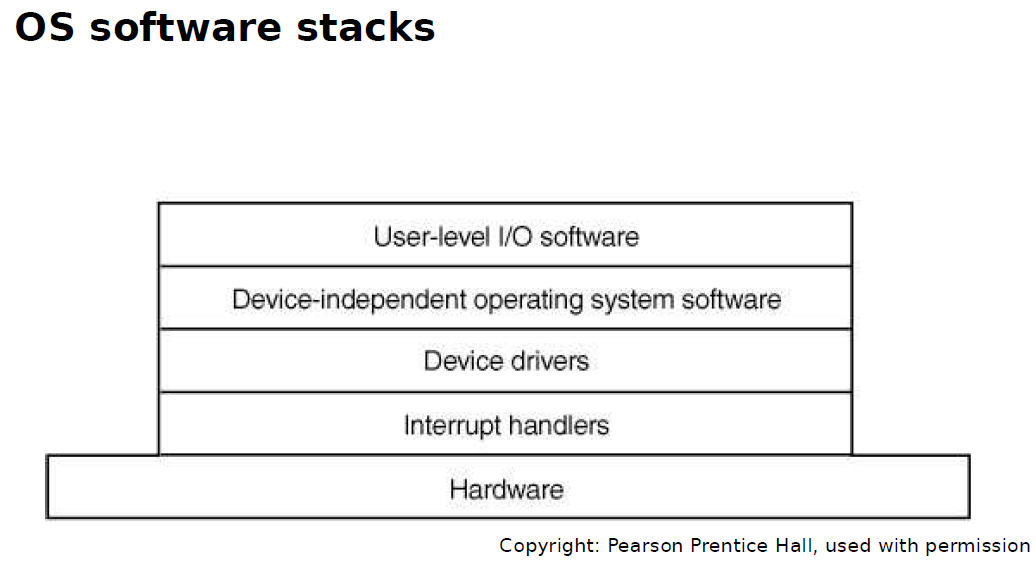
\includegraphics[width=8.0cm]{images/os-software-stack.png}
  \caption{Left: Taken from an Interwebs article called ``An Architecture for In-Vehicle Infotainment Systems''. Right: Taken from Sven's slides}
\end{figure}

HMI: Human-machine interface. Patrick is going to ignore this part, as this is not really shown in any other diagrams.

\subsection*{Application layer}
This is where people play The Sims(TODO: trademark symbol) and use MS Office, among other wonderful things.

Usually these rely on middleware instead of communicating directly with the OS. It is however entirely possible to communicate directly with the OS from this layer.

\subsection*{Middleware layer}
From Wikipedia: ``Middleware is a computer software that provides services to software applications beyond those available from the operating system. It can be described as ``software glue''. Middleware makes it easier for software developers to perform communication and input/output, so they can focus on the specific purpose of their application.''

\emph{OpenGL} and \emph{Miles Sound System} are examples of middleware.

\subsection*{OS layer}
The OS manages control and resources.

\subsection*{Hardware layer}
ZE MEMORY, PROCESSOR(S), STORAGE, I/O-DEVICES, AND SHIT.

Hidden away under several layers of abstraction, and developers cannot interact with this directly (except for in Exokernels).


\begin{figure}[H]
  \centering
  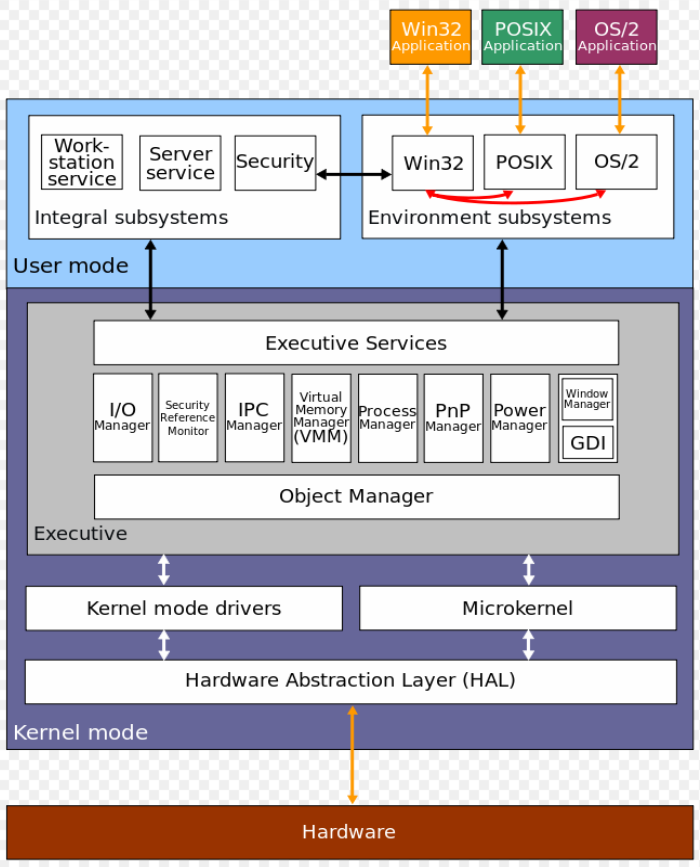
\includegraphics[width=8.0cm]{images/windows-nt-architecture.png}
  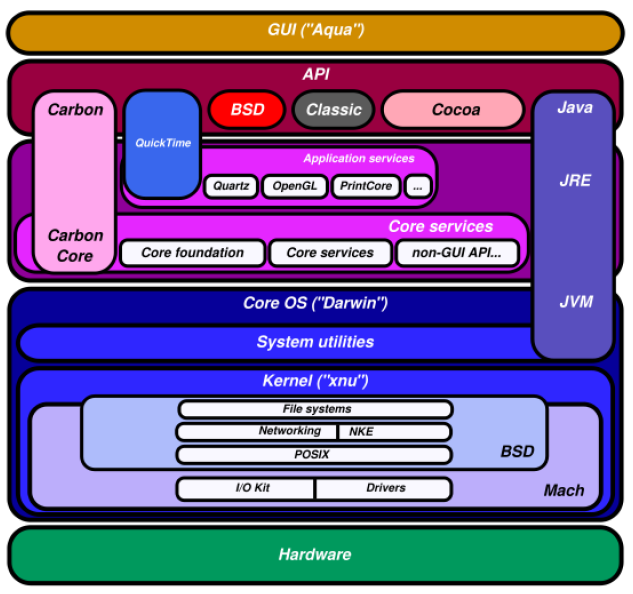
\includegraphics[width=8.0cm]{images/mac-os-x-architecture.png}
  \caption{The architectures of Windows NT and Mac OS X}
\end{figure}



\section{Key concepts}
\emph{20. Given reference literature, you can write down in text and in your own words definitions or explanations of the following concepts: Process; Address space; Interprocess communication; System call; Daemon; Thread; Critical section; Mutual exclusion; Semaphore; Mutex; Monitor; Condition variable; Message passing; Kernel mode; User mode; Pre-emtiveness; Race condition; Scheduling algorithm; System time; Device driver.}
\emph{24. Given reference literature, you can write down in text and in your own words definitions or explanations of the following concepts: Virtual machine; Virtual machine monitor; Atomic action; Swapping; Virtual memory; Paging; File system; File attribute.}
Given reference literature, you can write down in text and in your own words definitions or explanations of the following concepts:

\begin{description}
\item[Process Address space]
  The actual address space taken allocated to a process in a virtual address space.

\item[Interprocess communication]
  Can be done in numerous ways: files, message queues, semaphore, message passing, shared memory, pipes (IO), and more.

\item[System call]
  A program's request to the operating system to do an OS tasks

\item[Daemon]
  A process running in the background (``invisible''), can be a watchdog-like program, auto-updater, anti-virus, etc.

\item[Thread]
  Smallest ``unit'' known by the scheduler. Owned by a process. Threads of the same process share memory.

\item[Critical section]
  A piece of code that needs mutual exclusion. A critical \texttt{region} consists of multiple of these.

\item[Mutual exclusion]
  Ya kno dis

\item[Semaphore]
  P = request/take coconut, V = put coconut. Semaphore invariant: $\#P \le \#V + s$.

\item[Mutex]
  Binary semaphore, a simple lock/unlock mechanism

\item[Monitor]
  A construct (class, object, whatever) with mutual exclusion of methods

\item[Condition variable]
  A condition that a monitor can await to be signalled. In a Java monitor it's done via \texttt{wait} and \texttt{notify} and \texttt{notifyAll}. It's the mechanism by which a monitor can wait for a condition to be true without blocking the monitor.

\item[Message passing]
  Communication between objects in the same process or between different processes by use of so-called messages. Can be asynchronous or synchronous. Invoking a method on an object in Java is an example of message passing, and sending a signal from one process to another in unix with \texttt{kill} is another.

\item[Kernel mode]
  One of the two modes of operation of the CPU. In kernel mode all code executed is \textit{trusted} so it can access all memory, signal all processes, execute all instructions, etc.

\item[User mode]
  One of the two modes of operation of the CPU. In user mode code is not assumed to be \textit{trusted} so it is restricted to a certain memory space and possibly a limited subset of CPU instructions.

\item[Pre-emtiveness]
  A preemption happens when a process is suspended \textit{during} its execution, resulting in a \textit{context switch}, usually done by the scheduler. The intent is that the process will be resumed later.

\item[Race condition]
  Happens when two processes attempts to access/mutate a shared resources at the same time, such that unexpected behavior or corruption can occur.

\item[Scheduling algorithm]
  Algorithm that chooses which processes (or threads) to execute.

\item[System time]
  The computer's time ``counter''

\item[Device driver]
  Program that controls a hardware device and provides an interface to it (usually through the bus)

\item[Virtual machine]
  One machine providing multiple virtual machines (VM) to the next layer, such that multiple users can have their own, closed environment, while sharing the same resources.

\item[Virtual machine monitor]
  A hypervisor or virtual machine monitor (VMM) is a piece of computer software, firmware or hardware that creates and runs virtual machines.
\begin{figure}[H]
  \centering
  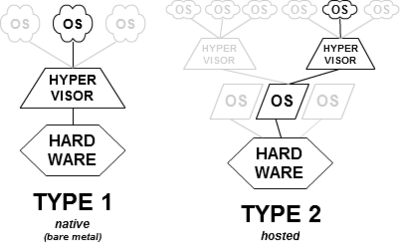
\includegraphics[scale=0.5]{images/hypervisor}
  \caption{Type-1 and type-2 hypervisors}
\end{figure}

\item[Atomic action]
  An instruction or set of instructions that cannot be interleaved by other processes, thus making it always completely done, or not started.

\item[Swapping]
  Memory management technique where a process is fully loaded into RAM to be run, and put back onto disk when idled.

\item[Virtual memory]
  Memory management technique in which a process is assigned \emph{virtual memory addresses} which are mapped by the operating system into physical memory locations, which could be either in RAM or on disk via paging. Allows programs to be run without being fully loaded into memory.

\item[Paging]
  Virtual memory is divided into fixed sized (512 bytes - 64KB) chunks called pages which are mapped to physical memory chunks (generally) of the same size. The MMU (memory management unit) translates addresses via a table.

\item[File system]
  A system by which the operating system distinguishes \emph{persistent} data stored on disk as separate units of coherent data, known as files.

\item[File attribute]
  Attributes attached to files such as being hidden, read-only, system critical, etc.

\end{description}


\section{Race conditions}
\emph{21. You can explain in your own words, in text and with your own examples how race conditions can occur in systems with multiple processors or systems with interrupts.}
%%% Local Variables:
%%% mode: latex
%%% TeX-master: "cheat-sheet"
%%% End:

Situations where two or more processes are reading or writing some shared data and the final result depends on who runs precisely when, are called \emph{race conditions}. Remember, processors are completely \emph{independent}.

A \emph{critical race} occurs when the order in which internal variables are changed determines the eventual state that the state machine will end up in.

A \emph{non-critical race} occurs when the order in which internal variables are changed does not alter the eventual state.

Race conditions creates \emph{Indeterministic} behavior, where the resulting state can not be determined.

Recreating a bug caused by a race condition might take some extreme set of parameters and are therefore very hard to find.

If shared variables, operations need to be \emph{synchronized}.

\subsection{Example}
\begin{align*}
\texttt{int x = 0;} \\ \\
&\textbf{P}_1 &\textbf{P}_2 \\
&\texttt{x = x + 1} &\texttt{x = 3}
\end{align*}

The final value of \texttt{x} can be 0 or 3.



\section{Mutual exclusion}
\emph{22. You can explain in your own words, in text and with your own commented examples, how busy wait methods can achieve mutual exclusion in systems with multiple CPUs.}
\emph{23. You can explain in your own words, in text and with your own commented examples, how blocking methods can achieve mutual exclusion in systems with multiple CPUs.}
% 22. You can explain in your own words, in text and with your own commented examples, how busy wait methods can achieve mutual exclusion in systems with multiple CPUs.
% 23. You can explain in your own words, in text and with your own commented examples, how blocking methods can achieve mutual exclusion in systems with multiple CPUs.

\subsection{Busy wait}
Uses the full resource of the thread to stay alive and continuously check for the critical section lock to become available.

Pseudo:
\begin{cpp}
int locked = 0;

void mutex_enter() {
  while (locked) { /* noop */ }
  locked = 1;
}

void mutex_exit() {
  locked = 0;
}
\end{cpp}

Usage
\begin{cpp}
mutex_enter();
/* critical section */
mutex_exit();
\end{cpp}

It is worth noting that one can also use the \texttt{TSL} (Test Set and Lock) or \texttt{CAS} (Compare And Swap) instructions to implement this.

\subsection{Blocking}
Puts the process to sleep and wakes it up from another process. Semaphores and monitors can do this. TODO: more?


%%% Local Variables:
%%% mode: latex
%%% TeX-master: "cheat-sheet"
%%% End:



\section*{Context switching}
Stores the state of the registers, as the rest will remain untouched by other processes (
TODO: mention individual 1) process address space and 2) call stack for each thread)


\section*{C - interrupts!}
TODO: fuck fuck fuck


\section*{C - storage classes (week 2)}
A storage class defines the scope and accesibility of defined variables.
\begin{description}
\item[auto] Default. Automatically freed when leaving block in which it's defined.
\item[extern] Defined outside current translation unit. Resolution of the variable or function is done at link-time.
\item[static] The visibility of the variable is restricted to current translation unit. Note that \texttt{static} can mean a bunch of things when used elsewhere.
\item[register] Prevents taking the address of a variable. Useful for instance to prevent accidentally returning a pointer to a function parameter. Does \textbf{not} mean that the variable is stored in a register, the compiler will decide on that.
\end{description}


\section*{C - qualifiers (week 3)}
\begin{description}
	\item[const] means that the variable may not be changed during the lifetime of the program.
	\item[volatile] means that the compiler is not allowed to optimize the usage of the variable.
	\item[restrict] ... something with pointer-accessing, and allows for better optimizations.
\end{description}



\section*{Memory layout (week3)}
TODO: (memory areas) How are they laid out? In what order Where in memory?


\section*{What is an OS? (week 5)}
\emph{From the slides:}

An OS is a \textbf{resource allocator}:
\begin{itemize}
	\item Manages all resources
	\item Decides between conflicting requests for efficient and fair resource use
\end{itemize}

An OS is a \textbf{control program}:
\begin{itemize}
	\item Controls execution of programs to prevent errors and improper use of the computer
\end{itemize}

... Although some systems do not even have these features.


\section*{Buzz}
%%% Local Variables:
%%% mode: latex
%%% TeX-master: "cheat-sheet"
%%% End:

\subsection*{Week 2 - C Programs}
%%% Local Variables:
%%% mode: latex
%%% TeX-master: "../cheat-sheet"
%%% End:

\subsubsection*{Programs}
\begin{itemize}
\item A Java program is a set of Classes
\item What does C programs consists of?
\item NB: There are major differences compared to Java
\end{itemize}

\paragraph{Answer}
See~\nameref{sec:o3}.

\subsubsection*{Preprocessor}
\begin{itemize}
  \item What is it and what can it do?
  \item How are translation units compiled?
  \item How are object files liked to form an executables?
    \begin{itemize}
      \item No details, just: “What is the purpose of the linker”? What does it do?
    \end{itemize}
\end{itemize}

\paragraph{Answer}
See~\nameref{sec:o3}.

\subsubsection*{Basic types}
List the basic types in C!

\paragraph{Answer}
\begin{itemize}
  \item \texttt{char}
  \item \texttt{int}
  \item \texttt{float}
  \item \texttt{double}
\end{itemize}

\subsubsection*{Storage classes}
What is the semantics of th following storage classes?
\begin{itemize}
  \item \texttt{auto}
  \item \texttt{extern}
  \item \texttt{static}
  \item \texttt{register}
\end{itemize}

\paragraph{Answer}
See~\nameref{sec:c-storage}.



\subsection*{Week 3 - C Programs part 2}
Memory - Buzz

\begin{itemize}
\item How is the memory in a computer typically organized?
  \begin{enumerate}
    \item How is it addressed?
    \item How does it look like to the processor?
    \item What memory areas do a program use?
    \item How are they laid out? In what order? Where in memory?
    \item Single threaded

  \end{enumerate}
\end{itemize}

Memory I - Buzz

Where do
\begin{itemize}
\item Global variables go?
\item How is it addressed?
\item How does it look like to the processor?
\end{itemize}

Pointers - Buzz

\begin{itemize}
\item Fundamentally, what is a pointer?
\item How is it represented?
\item How many bits are used?
\item Is type associated with pointers?
\item How do you do type casting?
\end{itemize}

Answers:

\begin{itemize}
\item  Fundamentally, pointers are represented as the smallest integer which can hold an address
– Describes an address and how to interpretate it
\item Represented using the (*) symbol. E.g. {\tt char *string; }
\item Like this: {\tt <++>ppi = (double ∗)pn; /∗ pn originally of type ( int ∗) ∗/ }
\end{itemize}



\subsection*{Week 5 - Operating Systems}
%%% Local Variables:
%%% mode: latex
%%% TeX-master: "../cheat-sheet"
%%% End:

\paragraph{Operating system, or OS, what is that?}

\begin{itemize}
\item Anything that supports the execution of a program/application or programming language
\item Operating systems are very often customized for a specific purpose (For example the iPhone OS or the engine controller in a car)
\item
  OS is a resource allocator
  \begin{itemize}
    \item Manages all resources
    \item Decides between conflicting requests for efficient and fair resource use
  \end{itemize}

  OS is a control program
  \begin{itemize}
    \item Controls execution of programs to prevent errors and improper use of the computer
  \end{itemize}
\end{itemize}

\paragraph{What resources are allocated through the OS? - How does it control programs?}

\begin{itemize}
\item Memory
\item CPU time
\item privileges
\item I/O
\end{itemize}



\subsection*{Week 6 - Processes}
%%% Local Variables:
%%% mode: latex
%%% TeX-master: "cheat-sheet"
%%% End:

\subsection*{Week 6 - Processes}
\textbf{intro}
\begin{itemize}
\item What does a program use during its lifetime?
\begin{itemize}
\item Hint: what does a program need to execute?
\end{itemize}
\end{itemize}
\\
\textbf{Buzz: What is a system call}
\\
\textbf{System Calls}
\begin{itemize}
\item Programming interface to the sercices proided by the OS.
\begin{itemize}
\item Processes $\rightarrow$ the operating system
\end{itemize}
\item Mostly accessed by programs via a higlh-level Application Program Interface (API) rather than direct system call use.
\item Three most common APIs are Win32 API for windows, POISX API for POISX API for POISX-Based systems (includi´ng virtually all versions of UNIX, Linux, and Mac OS X), and Java API for the Java virtual machine (JVM).
\end{itemize}
\\
\textbf{How Are system calls implemented?}
\begin{itemize}
\item What are the steps in executing a system call?
\item How are parameters to system calls passed to the operating system?
\item Does the type and organization of the operating system matter?
\item Draw a figure to help you.
\end{itemize}
\textbf{System Call Implementation}
\begin{itemize}
\item Typically, a number associated with each system call.
\item The system call interface invokes intended system call in OS kernel and returns status of the system call and any return values.
The caller need know nothing about how the systemm call is implemented.
\begin{itemize}
\item Just needs to obay API and understand what the OS will do
\end{itemize}
\end{itemize}


\subsection*{Week 7 - Scheduling}
%%% Local Variables:
%%% mode: latex
%%% TeX-master: "cheat-sheet"
%%% End:

\subsubsection*{Forms of scheduling}
One form of scheduling is to map threads, and hence processes, to CPUs.

What are other forms?

\subsubsection*{How do you do a context switch?}


\subsubsection*{Bonus: Fragmentation}
\begin{description}
\item[External Fragmentation]: total memory space exists to satisfy a request, but it is not contiguous
\item[Internal Fragmentation]: allocated memory block may be slightly larger than requested memory
\end{description}
Fragmentation \texttt{will} happen


\subsection*{Week 12 - Virtual Machines}
\subsection*{Week 12 - Virtual Machines}
\subsubsection*{Why virtual machines and virtual machine monitors?}

\begin{itemize}
	\item You have plenty of installations...
	\begin{itemize}
		\item Servers
		\item Operating systems versions	
	\end{itemize}
	
	\item ... but not much hardware
	\begin{itemize}
		\item Hardware == Energy == Money
		\item Many installations are idle
	\end{itemize}
	\item Usage scenario: Web hosting
	\begin{itemize}
		\item Fewer machines to manage
		\item Hopefully not less reliable or less secure	
	\end{itemize}
	\item Hypervisor can control a number of guest operating systems
\end{itemize}

\subsubsection*{Migration}
``One advantage of using virtual machines is that you can move a virtual machine from one hardware machine to another. How could one do that?''

Image that you have two machines; \emph{Machine A} and \emph{Machine B}. The user using is running \emph{Machine A}, but the overall system decides that the virtual machine should be moved to \emph{Machine B} (probably due to \emph{Machine A} is failing).

The job is to make the transition as smooth as possible for the user. This is achieved by copying all of the memory from \emph{Machine A} to \emph{Machine B}. But this is not done in a random manner:
\begin{enumerate}
	\item Firstly, the memory of the processes \emph{not} used by the user is copied from \emph{Machine A} to \emph{Machine B}
	\item When all but the critical memory has been copied (after a some seconds), the process will shortly freeze as the last data it is moved from \emph{Machine A} to \emph{Machine B}
	\item Now the user's entire virtual machine is running on \emph{Machine B}
\end{enumerate}



\end{document}
